\documentclass[journal,12pt,twocolumn]{IEEEtran}
%
\usepackage{setspace}
\usepackage{multicol}
\usepackage{gensymb}
\usepackage{enumerate}
\usepackage{xcolor}
\usepackage{caption}
%\usepackage{subcaption}
%\doublespacing
\singlespacing
%\usepackage{epstopdf}
%\usepackage{graphicx}
%\usepackage{amssymb}
%\usepackage{relsize}
\usepackage[cmex10]{amsmath}
\usepackage{mathtools}
%\usepackage{amsthm}
%\interdisplaylinepenalty=2500
%\savesymbol{iint}
%\usepackage{txfonts}
%\restoresymbol{TXF}{iint}
%\usepackage{wasysym}
\usepackage{amsthm}
\usepackage{mathrsfs}
\usepackage{txfonts}
\usepackage{stfloats}
\usepackage{cite}
\usepackage{cases}
\usepackage{subfig}
%\usepackage{xtab}
\usepackage{longtable}
\usepackage{multirow}
%\usepackage{algorithm}
%\usepackage{algpseudocode}
%\usepackage{enumitem}
\usepackage{mathtools}
\usepackage{iithtlc}
%\usepackage[framemethod=tikz]{mdframed}
\usepackage{listings}
\usepackage{amsmath}
\usepackage{polynomial}
\usepackage{url}
\def\UrlBreaks{\do\/\do-}
%\usepackage{stmaryrd}


%\usepackage{wasysym}
%\newcounter{MYtempeqncnt}
\DeclareMathOperator*{\Res}{Res}
%\renewcommand{\baselinestretch}{2}
\renewcommand\thesection{\arabic{section}}
\renewcommand\thesubsection{\thesection.\arabic{subsection}}
\renewcommand\thesubsubsection{\thesubsection.\arabic{subsubsection}}

\renewcommand\thesectiondis{\arabic{section}}
\renewcommand\thesubsectiondis{\thesectiondis.\arabic{subsection}}
\renewcommand\thesubsubsectiondis{\thesubsectiondis.\arabic{subsubsection}}

% correct bad hyphenation here
\hyphenation{op-tical net-works semi-conduc-tor}

\lstset{
language=Python,
frame=single, 
breaklines=true
}

%\lstset{
	%%basicstyle=\small\ttfamily\bfseries,
	%%numberstyle=\small\ttfamily,
	%language=python,
	%backgroundcolor=\color{white},
	%%frame=single,
	%%keywordstyle=\bfseries,
	%%breaklines=true,
	%%showstringspaces=false,
	%%xleftmargin=-10mm,
	%%aboveskip=-1mm,
	%%belowskip=0mm
%}

%\surroundwithmdframed[width=\columnwidth]{lstlisting}


\begin{document}
%

\theoremstyle{definition}
\newtheorem{theorem}{Theorem}[section]
%\newtheorem{problem}{Problem}[section]
\newtheorem{problem}{Problem}
\newtheorem{proposition}{Proposition}
%\newtheorem{proposition}{Proposition}[section]
\newtheorem{lemma}{Lemma}[section]
\newtheorem{corollary}[theorem]{Corollary}
\newtheorem{example}{Example}[section]
%\newtheorem{definition}{Definition}[section]
\newtheorem{definition}{Definition}
%\newtheorem{definition}{Definition}
%\newtheorem{algorithm}{Algorithm}[section]
%\newtheorem{cor}{Corollary}
\newcommand{\BEQA}{\begin{eqnarray}}
\newcommand{\EEQA}{\end{eqnarray}}
\newcommand{\define}{\stackrel{\triangle}{=}}

\bibliographystyle{IEEEtran}
%\bibliographystyle{ieeetr}

\providecommand{\nCr}[2]{\,^{#1}C_{#2}} % nCr
\providecommand{\nPr}[2]{\,^{#1}P_{#2}} % nPr
\providecommand{\mbf}{\mathbf}
\providecommand{\pr}[1]{\ensuremath{\Pr\left(#1\right)}}
\providecommand{\qfunc}[1]{\ensuremath{Q\left(#1\right)}}
\providecommand{\sbrak}[1]{\ensuremath{{}\left[#1\right]}}
\providecommand{\lsbrak}[1]{\ensuremath{{}\left[#1\right.}}
\providecommand{\rsbrak}[1]{\ensuremath{{}\left.#1\right]}}
\providecommand{\brak}[1]{\ensuremath{\left(#1\right)}}
\providecommand{\lbrak}[1]{\ensuremath{\left(#1\right.}}
\providecommand{\rbrak}[1]{\ensuremath{\left.#1\right)}}
\providecommand{\cbrak}[1]{\ensuremath{\left\{#1\right\}}}
\providecommand{\lcbrak}[1]{\ensuremath{\left\{#1\right.}}
\providecommand{\rcbrak}[1]{\ensuremath{\left.#1\right\}}}
\theoremstyle{remark}
\newtheorem{rem}{Remark}
\newcommand{\sgn}{\mathop{\mathrm{sgn}}}
\providecommand{\abs}[1]{\left\vert#1\right\vert}
\providecommand{\res}[1]{\Res\displaylimits_{#1}} 
\providecommand{\norm}[1]{\lVert#1\rVert}
\providecommand{\mtx}[1]{\mathbf{#1}}
\providecommand{\mean}[1]{E\left[ #1 \right]}
\providecommand{\fourier}{\overset{\mathcal{F}}{ \rightleftharpoons}}
%\providecommand{\hilbert}{\overset{\mathcal{H}}{ \rightleftharpoons}}
\providecommand{\system}{\overset{\mathcal{H}}{ \longleftrightarrow}}
	%\newcommand{\solution}[2]{\textbf{Solution:}{#1}}
\newcommand{\solution}{\noindent \textbf{Solution: }}
\providecommand{\dec}[2]{\ensuremath{\overset{#1}{\underset{#2}{\gtrless}}}}
%\numberwithin{equation}{section}
\numberwithin{equation}{problem}

%\numberwithin{problem}{subsection}
%\numberwithin{definition}{subsection}
\makeatletter
\@addtoreset{figure}{problem}
\makeatother

\let\StandardTheFigure\thefigure
%\renewcommand{\thefigure}{\theproblem.\arabic{figure}}
\renewcommand{\thefigure}{\theproblem}


%\numberwithin{figure}{subsection}

\def\putbox#1#2#3{\makebox[0in][l]{\makebox[#1][l]{}\raisebox{\baselineskip}[0in][0in]{\raisebox{#2}[0in][0in]{#3}}}}
     \def\rightbox#1{\makebox[0in][r]{#1}}
     \def\centbox#1{\makebox[0in]{#1}}
     \def\topbox#1{\raisebox{-\baselineskip}[0in][0in]{#1}}
     \def\midbox#1{\raisebox{-0.5\baselineskip}[0in][0in]{#1}}

\vspace{3cm}

\title{ 
\logo{
Algebraic and Transcendental Equations
}
}

\author{G V V Sharma$^{*}$ %<-this  stops a space
\thanks{*The author is with the Department
of Electrical Engineering, IIT, Hyderabad
502285 India e-mail: gadepall@iith.ac.in. All material in the manuscript is released under GNU GPL.  Free to use for all.}% <-this % stops a space
}



% make the title area
\maketitle

%\newpage

%\tableofcontents


\IEEEpeerreviewmaketitle

\bigskip

\begin{abstract}
Through examples, this manual introduces methods for solving 
algebraic and transcendental equations like the
bisection method, the method of false position,  the iteration method
and the Newton-Raphson method
Python codes are provided for all these methods.
\end{abstract}
%
\section{Fixed Point Iteration}
\begin{theorem}
Consider the  equation 
\begin{equation}
\label{eq:fpi}
x = g(x)
\end{equation}
%
If $\abs{g^{\prime}(x) \leqslant K < 1}$, then it is possible to frame a difference
equation
%
\begin{equation}
x_{n+1} = g(x_n)
\end{equation}
%
to solve \eqref{eq:fpi} \cite{kreyszig}.
\end{theorem}
%
\begin{problem}
Sketch
\begin{equation}
\label{eq:fpi_example}
x^3 + x - 1 =0
\end{equation}
%
\end{problem}
\solution The following code generates the Fig. \ref{fig:fpi_example}
\lstinputlisting{./codes/fpi_example.py}
\begin{figure}[!h]
\centering
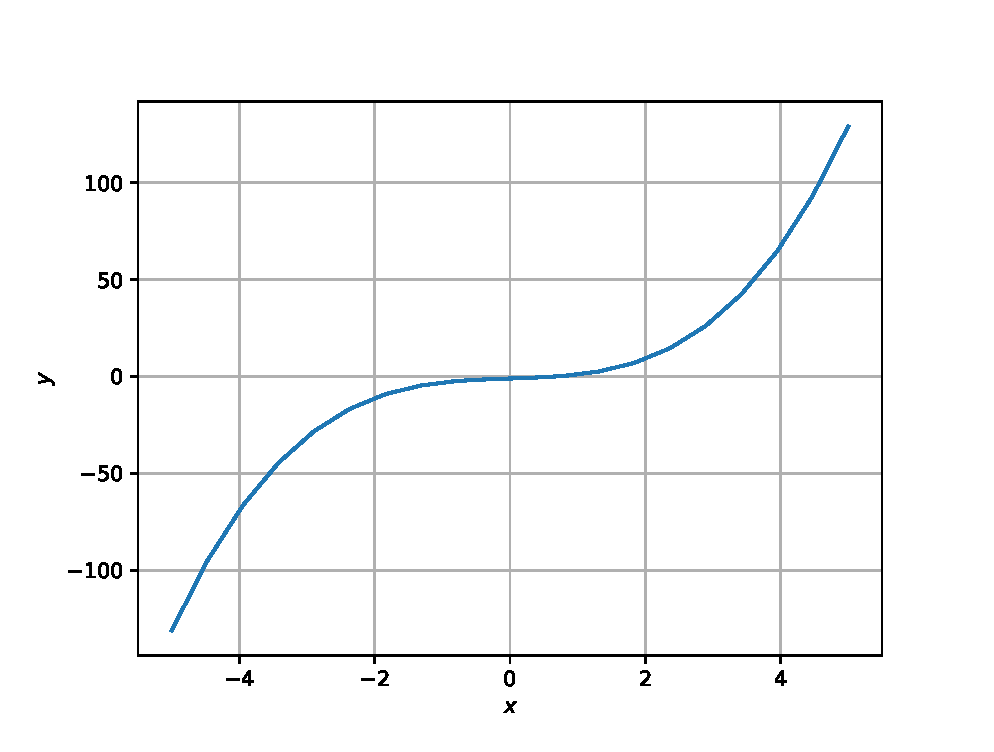
\includegraphics[width=\columnwidth]{./figs/fpi_example.eps}
\caption{The solution is at the point where the function meets the $X$-axis.}
\label{fig:fpi_example}
\end{figure}

\begin{problem}
Obtain the difference equation for \eqref{eq:fpi_example}
%
by iteration.
\end{problem}
%
\solution  Expressing \eqref{eq:fpi_example} as
\begin{equation}
x  = \frac{1}{1+x^2},
\end{equation}
%
the difference equation
%
\begin{equation}
\label{eq:fpi_example_diff}
x_{n+1}  = \frac{1}{1+x_n^2},
\end{equation}
%
is obtained.
%
\begin{problem}
Solve \eqref{eq:fpi_example_diff}.
\end{problem}
%
\solution The following script computes \eqref{eq:fpi_example_diff} resulting in
\begin{equation}
x = 0.6823278038681895
\end{equation}
\lstinputlisting{./codes/fpi.py}

\section{Newton-Ralphson Method}
\begin{problem}
Obtain the difference equation for solving 
%
%
\begin{equation}
\label{eq:newton}
f(x) = 0.
\end{equation}
\end{problem}
\solution From \cite{newton}, the desired difference equation is
%
\begin{equation}
\label{eq:newton_diff}
 x_{n+1}=x_{n}-{\frac {f(x_{n})}{f^{\prime}(x_{n})}}
\end{equation}
%
\begin{problem}
Solve \eqref{eq:fpi_example} using \eqref{eq:newton_diff} for 4 iterations.
\end{problem}
\solution Using the fact that
%
\begin{equation}
f^{\prime}(x) = 3x^2+1,
\end{equation}
%
The following script computes \eqref{eq:newton_diff} resulting in
\begin{equation}
x = 0.6823278039465127
\end{equation}
\lstinputlisting{./codes/newton.py}
%
\begin{problem}
Compare the Newton-Ralphson method with the Iteration method.
\section{Bisection Method}
\begin{theorem}
\label{them:bisection}
Consider \eqref{eq:fpi_example} and Fig. \ref{fig:fpi_example}.  Choose a points $a,b$ for which $f(a) < 0, f(b) > 0$.  Find $c_0 = \frac{a+b}{2}$.  If $f(c_0) < 0, c_1 = \frac{c_1+b}{2} $, else $c_1 = \frac{a+ c_1 }{2}$.  Similarly choose $c_2, c_3,\dots$.  For sufficiently large iterations, $c_n$ will coverge to a root of $f(x)$. Note that this will happen only if $f(x)$ is continuous in $\brak{a,b}$ \cite{bisection}.
\end{theorem}
\end{problem}
%
\begin{problem}
Solve \eqref{eq:fpi_example} using Theorem \ref{them:bisection}.
\end{problem}
\solution From Fig. \ref{fig:fpi_example}, $f(-1) < 0$ and $f(1) > 0$.  Choosing $a = -1, b = 1$ initially,
the following script computes the solution resulting in
\begin{equation}
x = 0.6823278038280183
\end{equation}
for 50 iterations.
\lstinputlisting{./codes/bisection.py}
%
\section{Method of False Position}
%
\begin{theorem}
\label{them:false_position}
Consider \eqref{eq:fpi_example}.  Choose a points $a,b$ for which $f(a) < 0, f(b) > 0$.  
Find \cite{falsepos}
\begin{equation}
c_{k}=b_{k}-f(b_{k}){\frac {(b_{k}-a_{k})}{f(b_{k})-f(a_{k})}}
\end{equation}
If $f(c_k) < 0, a_k = c_k $, else $b_k = c_k$.  For sufficiently large iterations, $c_n$ will coverge to a root of $f(x)$. Note that this will happen only if $f(x)$ is continuous in $\brak{a,b}$.
\end{theorem}
%
\begin{problem}
Solve \eqref{eq:fpi_example} using Theorem \ref{them:false_position}.
\end{problem}
\solution From Fig. \ref{fig:fpi_example}, $f(-1) < 0$ and $f(1) > 0$.  Choosing $a = -1, b = 1$ initially,
the following script computes the solution resulting in
\begin{equation}
x = 0.6823278038280193
\end{equation}
for 50 iterations.
\lstinputlisting{./codes/false_position.py}
%
\begin{problem}
What is the difference between the bisection method and the method of false position?
\end{problem}
\bibliography{IEEEabrv,gvv_eq}
\end{document}


